\begin{appendices}

\chapter{Appendix A}
	 % \includecode{codes/default.vcl}
	 \lstset{basicstyle=\footnotesize\ttfamily}
	 \lstinputlisting[frame=single,linewidth=15cm,breaklines, caption=Varnish Configuration ]{codes/default.vcl}

\chapter{Appendix B}
	 
	\begin{figure}[h]
    	\centering
		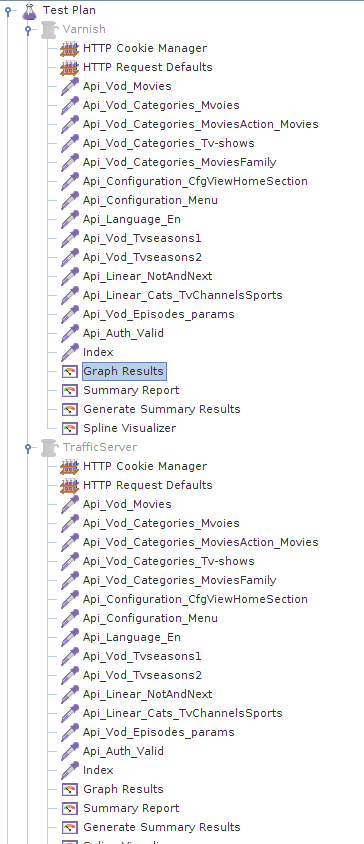
\includegraphics[width=10cm,height=15cm,keepaspectratio]{images/jmeter_conf.png}
    	\caption{Jmeter Configuration}
    	\label{fig:jmeter_conf}
	\end{figure}

\chapter{Appendix C}
	 % \includecode{codes/default.vcl}
	 \lstset{basicstyle=\footnotesize\ttfamily}
	 \lstinputlisting[frame=single,linewidth=15cm,breaklines, caption=Content Provider Dictionary ]{codes/content_provider.json}


\chapter{Appendix D}

\begin{lstlisting}[frame=single,linewidth=15cm,breaklines=true,caption=HQL usage]
	var parser = new HQLParser();
	var requestJson = parser
		  .select('category_movies', 'accedo.ovp.categories.movies')
		  .setConstantParameter('id', ['movies-action'])
		  .setQueryParameter('pageSize', 2)
		  .select('category_tvshows', 'accedo.ovp.categories.tvshows')
		  .setConstantParameter('id', ['tv_shows_comedy'])
		  .setQueryParameter('pageSize', 2)
		  .select('episodes', 'accedo.ovp.episodes')
		  .setQueryParameter('pageSize', 2)
		  .select('tvshow', 'accedo.ovp.tvshow')
		  .setParentParameter('id', 'episodes', 'entries.metadata', 'value')
		  .addConstraints('id', [{key: "name", value: "VOD$tvShowId"}])
		  .select('tvseason', 'accedo.ovp.tvseason')
		  .setParentParameter('id', 'episodes', 'entries.metadata', 'value')
		  .addConstraints('id', [{key: "name", value: "VOD$tvSeasonId"}])
		  .build();

\end{lstlisting}

\end{appendices}
